\documentclass[12pt,a4paper]{article}
\usepackage{tikz}
\usepackage{pgfplots}
\usepackage{pgf-pie}
\usetikzlibrary{shapes.geometric, shapes.multipart, arrows.meta, positioning, fit, calc, backgrounds}
\pgfplotsset{compat=1.18}

\begin{document}

\section*{Inter-Process Communication (Clean Architecture)}

\begin{figure}[htbp]
\centering
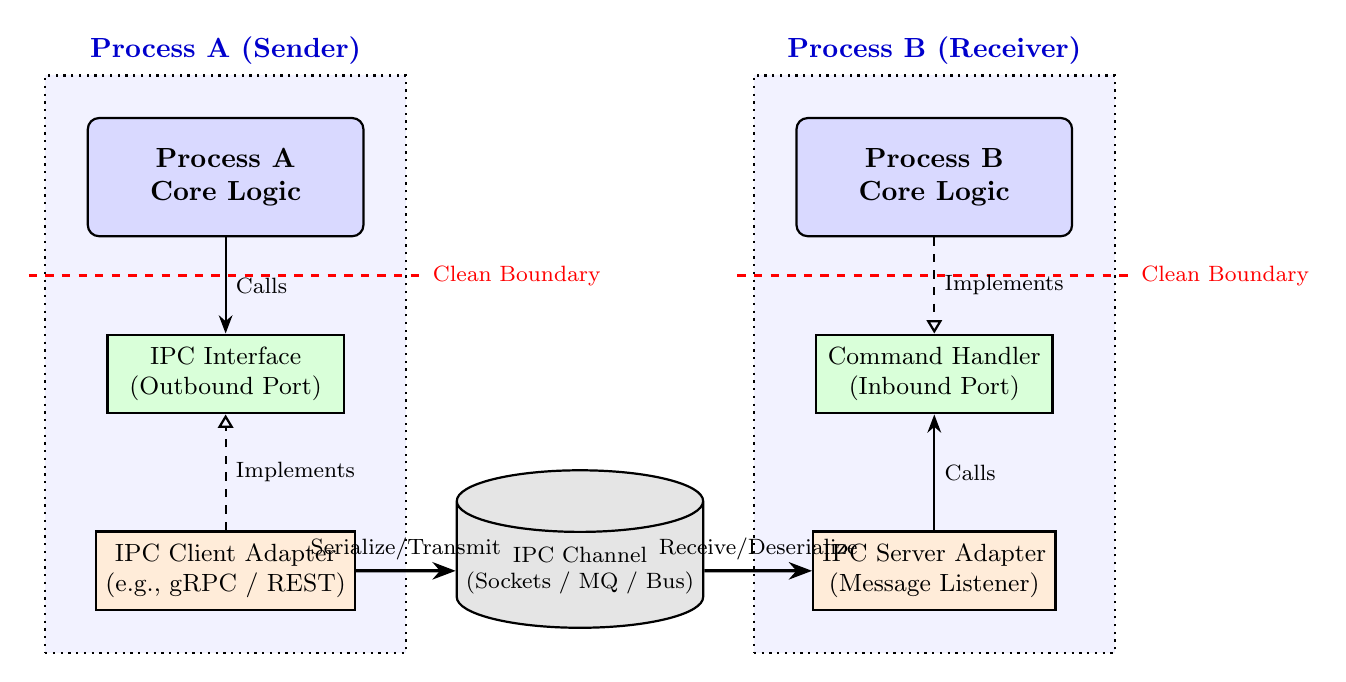
\begin{tikzpicture}[
  node distance=1.5cm,
  core/.style={rectangle, rounded corners, draw, thick, fill=blue!15, minimum width=3.5cm, minimum height=1.5cm, align=center, font=\bfseries},
  port/.style={rectangle, draw, thick, fill=green!15, minimum width=3cm, minimum height=1cm, align=center, font=\small},
  adapter/.style={rectangle, draw, thick, fill=orange!15, minimum width=3cm, minimum height=1cm, align=center, font=\small},
  ipc/.style={cylinder, draw, thick, fill=gray!20, aspect=0.25, minimum height=2cm, minimum width=2.5cm, align=center, shape border rotate=90, font=\footnotesize},
  arr/.style={->, -{Stealth}, thick},
  impl/.style={-{Triangle[open]}, dashed, thick} % UML Realization/Implementation arrow
]

% -------------------------
% PROCESS A (CLIENT)
% -------------------------
\node[core] (coreA) at (0, 0) {Process A\\Core Logic};
\node[port] (portA) at (0, -2.5) {IPC Interface\\(Outbound Port)};
\node[adapter] (adapterA) at (0, -5) {IPC Client Adapter\\(e.g., gRPC / REST)};

% Clean Architecture Boundary Line for Process A
\draw[dashed, red, thick] (-2.5, -1.25) -- (2.5, -1.25) node[right, font=\footnotesize, text=red] {Clean Boundary};

% Dependencies
\draw[arr] (coreA) -- node[right, font=\footnotesize] {Calls} (portA);
\draw[impl] (adapterA) -- node[right, font=\footnotesize] {Implements} (portA);

% -------------------------
% IPC CHANNEL
% -------------------------
\node[ipc] (channel) at (4.5, -5) {IPC Channel\\(Sockets / MQ / Bus)};

% Network communication
\draw[arr, very thick] (adapterA) -- node[above, font=\footnotesize] {Serialize/Transmit} (channel);

% -------------------------
% PROCESS B (SERVER)
% -------------------------
\node[adapter] (adapterB) at (9, -5) {IPC Server Adapter\\(Message Listener)};
\node[port] (portB) at (9, -2.5) {Command Handler\\(Inbound Port)};
\node[core] (coreB) at (9, 0) {Process B\\Core Logic};

% Clean Architecture Boundary Line for Process B
\draw[dashed, red, thick] (6.5, -1.25) -- (11.5, -1.25) node[right, font=\footnotesize, text=red] {Clean Boundary};

% Network communication
\draw[arr, very thick] (channel) -- node[above, font=\footnotesize] {Receive/Deserialize} (adapterB);

% Dependencies
\draw[arr] (adapterB) -- node[right, font=\footnotesize] {Calls} (portB);
\draw[impl] (coreB) -- node[right, font=\footnotesize] {Implements} (portB);

% -------------------------
% BACKGROUND PROCESS BOXES
% -------------------------
\begin{pgfonlayer}{background}
  % Box around Process A
  \node[draw, thick, dotted, fill=blue!5, fit=(coreA) (portA) (adapterA), inner sep=15pt, label={[font=\bfseries, text=blue!80!black]above:Process A (Sender)}] {};
  
  % Box around Process B
  \node[draw, thick, dotted, fill=blue!5, fit=(coreB) (portB) (adapterB), inner sep=15pt, label={[font=\bfseries, text=blue!80!black]above:Process B (Receiver)}] {};
\end{pgfonlayer}

\end{tikzpicture}
\end{figure}
\end{document}
